\section{Risultati della stabilizzazione}

\subsection{Validità della linearizzazione}
Il sistema non è lineare, quindi mi aspetto che il regolatore lineare quadratico sia
effettivo solamente entro un certo angolo iniziale\footnotemark da $\theta = 0$.
Per ottenere una stima dell'intervallo di validità, espando l'equazione del
moto~\eqref{eq:moto-carrello-theta} in serie di Taylor fino al terzo ordine,
fissando $\dot \theta = 0$.
Sostituendo i valori numerici dei parametri, ottengo
\begin{equation*}
    \frac {\ddot \theta} {\text{cost.}} \approx 4 \theta + \theta^3 + \mathcal O(\theta^4).
\end{equation*}
Mi aspetto che l'approssimazione sia valida quando il termine in $\theta^3$ è
molto minore del termine in $\theta$
\begin{equation}
    \frac{4\theta} {\theta^3} \gg 1.
    \label{eq:rapporto-theta}
\end{equation}

Ho simulato il sistema usando il regolatore lineare quadratico
con diverse condizioni iniziali e ho trovato che
il sistema smette di essere controllabile quando $|\theta(0)| = \theta_{\max} \approx 1.1$,
quindi quando il rapporto nella~\eqref{eq:rapporto-theta} si avvicina a $3.3$.
I coefficienti di costo $r_{11}$ e $q_{11}$ non influiscono
direttamente sul range di controllabilità, ma possono alterare
il comportamento del sistema quando le condizioni iniziali sono
vicine a $\theta = \theta_{\max}$.
Illustro questo fatto in \autoref{fig:occasional-blowup}.

Attraverso le simulazioni ho osservato che l'unica variabile
significativa per la controllabilità è $\theta$.
Posso stimare ugualmente un valore massimo per le altre
variabili considerando l'energia che il sistema ha nello stato
\begin{equation*}
    \b x = (0, 0, \theta_{\max}, 0)
\end{equation*}
e stimando che, perchè il sistema sia controllabile,
l'energia debba essere minore di questo valore.

\begin{figure}
    \vskip 0pt
    \centering
    \begin{subfigure}[t]{0.48\textwidth}
        \centering
        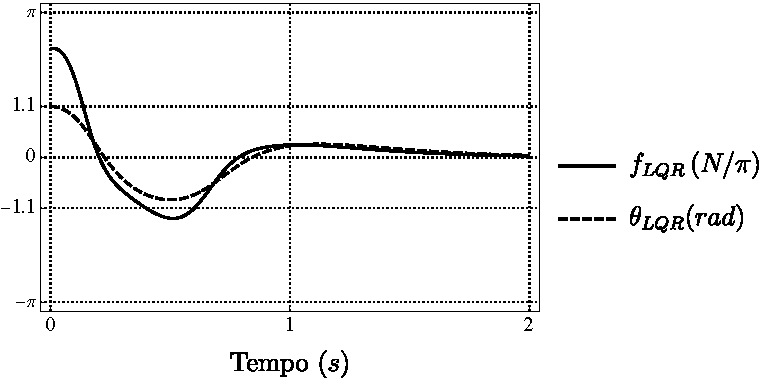
\includegraphics[width=\textwidth]{assets/occasional-blowup-r1}
        \caption{$r_{11} = 1$. Il sistema riesce a tornare a $\b x = \b 0$.}
        \label{eq:does-not-blowup}
    \end{subfigure}
    \hfill
    \begin{subfigure}[t]{0.48\textwidth}
        \centering
        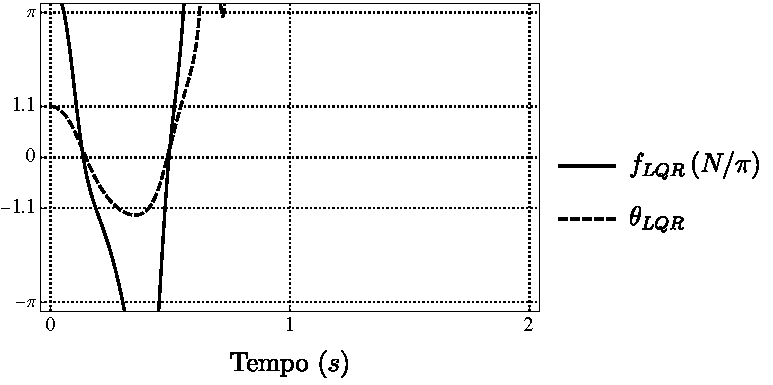
\includegraphics[width=\textwidth]{assets/occasional-blowup-r.1}
        \caption{$r_{11} = .1$. Il sistema risponde troppo
            aggressivamente, $\theta$ supera $\theta_{\max}$ e la soluzione diverge.}
        \label{eq:does-blowup}
    \end{subfigure}
    \caption[Dipendenza delle soluzioni dal costo]{
        Dipendenza delle soluzioni dai coefficienti della funzione costo
        per condizioni iniziali vicine a $\theta = 0$.
        Le due simulazioni nelle Figure~\ref{eq:does-not-blowup} e~\ref{eq:does-blowup}
        hanno entrambe come condizione iniziale $\b x = (0, 0, 1, 0)$ ma
        hanno diversi coefficienti $r_{11}$ per la funzione costo.
    }
    \label{fig:occasional-blowup}
\end{figure}

\footnotetext{
    $q$ e $\dot q$ non compaiono nelle equazioni del moto~\eqref{eq:moto-sistema},
    quindi non sono rilevanti per la validità della linearizzazione. Per
    ora considero $\dot \theta(0) = 0$.
}




\subsection{Ottimalità del controllo}

\subsection{Stabilizzazione del sistema reale}